%==============================================================

\section{Big Data Framework Spark}\label{bds1}

After the features are extracted, the next step is to load the feature files into the HDFS.
All feature files of the same type get merged into one large file. For the about 114000 songs these feature files sum up to about 11.2 GB (see figure \ref{filesize}). 

\begin{figure}[htbp]
	\centering
	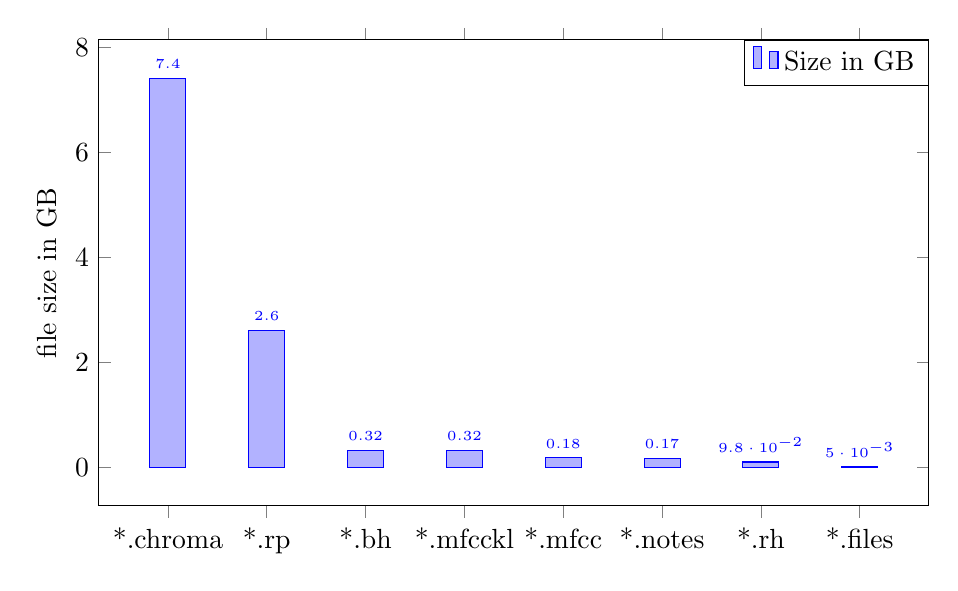
\begin{tikzpicture}
		\begin{axis}[
		    width=\textwidth,height=75mm,% <- added
		    x tick label style={/pgf/number format/1000 sep=},
      		xticklabels={ ,  , *.chroma, *.rp, *.bh, *.mfcckl, *.mfcc, *.notes, *.rh, *.files}, 
		    ylabel=file size in GB,
		    %enlargelimits=0.05,% <- commented, default is .1
		    legend style={
		      at={(1,1)},
		      anchor=north east,% <- changed
		      %legend columns=-1% <- commented
		    },
		    nodes near coords,
		    every node near coord/.append style={font=\tiny},
		    %nodes near coords align={vertical},% <- commented, default
		    ybar=0pt,%<- changed
		    bar width=13pt% <- added
		  ]
		  \addplot
		    coordinates {(1,7.400) (2,2.600) (3,0.324) (4,0.324) (5,0.177) (6,0.174) (7,0.098) (8,0.005)};
		  \legend{Size in GB}
		\end{axis}
	\end{tikzpicture}
	\caption{File sizes}
	\label{filesize}
\end{figure}

\noindent Large streaming platforms like Spotify give access to about 30 million songs in their databases. At this scale, the feature files would be approximately sum up to about 3 TB.\\

\subsubsection{underlying hardware}

The first tests with Spark were performed on a single PC with 4 CPU cores (8 with HT) (Intel Core i7-3610QM CPU, 2.30GHz × 4) running Spark 2.4.0.\\ The cluster test were performed on the ARA- Cluster, that offers 16 compute-nodes with 32 CPU-cores (Dual Socket, 2 x Intel Xeon "Scalable" 6140, 2.30 GHz x 18) per node (72 with HT) and 192GB of RAM. The cluster was running an older version of Spark (1.6.0)\\

\subsection{workflow}

\begin{figure}[htbp]
	\centering
	\framebox{\parbox{1\textwidth}{ 	
		\centering
		\ \\
		%\smartdiagramset{set color list={blue!40!white, blue!40!white,blue!40!white, blue!40!white, blue!40!white, blue!40!white}}
		\tikzset{priority arrow/.append style={rotate=180,anchor=0,xshift=30,}}			
		\smartdiagram[priority descriptive diagram]{5) return result, 4) joining results, 3) distance scaling, 2) distance computation, 1) data preparation and caching} \\
		\caption{Workflow Spark}
		\label{workflowspark}
	}}
\end{figure}
\FloatBarrier

\subsection{Data preparation}

The features are stored in text files as described in chapter \ref{sumfeat}. Due to the fact that the features were extracted in parallel and in batches of only a few songs, each of the feature files only contain the features of a small number of songs. Because many small files are inefficient to process with Spark \cite[p. 153]{sparkbook1} all files containing the same feature type are merged to one large file, before being loaded into the HDFS. By loading larger files into the HDFS, the partitioning into data blocks is performed according to the standard parameters of the HDFS (e.g. 128 MB partitions). Additional repartitioning on the cluster is later performed with Spark by using the \lstinline{rdd.repartition(repartition\_count)} command. 
Finally to work with the features a few transformations have to be performed on the data. For example the extracted note values are stored as lists of integer numbers, each representing a certain note. To compare these using the Levenshtein distance, these lists are converted into strings. 

\begin{pythonCode}[frame=single,label={lst:prep1},caption={notes preprocessing},captionpos=b]
chroma = sc.textFile("features/out[0-9]*.notes").repartition(repartition_count)
chroma = chroma.map(lambda x: x.split(';'))
chroma = chroma.map(lambda x: (x[0], x[1], x[2], x[3].replace("0",'A').replace("1",'B').replace("2",'C').replace("3",'D').replace("4",'E').replace("5",'F').replace("6",'G').replace("7",'H').replace("8",'I').replace("9",'J').replace("10",'K').replace("11",'L'))).map(lambda x: (x[0], x[1], x[2], x[3].replace(',','').replace(' ','')))
df = spark.createDataFrame(chroma, ["id", "key", "scale", "notes"])
\end{pythonCode}

\noindent All the other features are stored as lists of floats and have to be converted to vectors. The Spark ML library and the older MLlib library offer sparse and dense vectors as a data type. The only feature type that contains a lot of zeros and where sparse vectors could improve performance is the beat histogram. But compared to other features like the chromagram they are relatively small (with a length of only 200 values) so all lists including the beat histograms are converted to dense vectors by calling \lstinline{Vectors.dense(l)}. An example is given for the rhythm pattern features in code snippet \ref{lst:rpp}.

\begin{pythonCode}[frame=single,label={lst:rpp},caption={rp preprocessing},captionpos=b]
from pyspark.mllib.linalg import Vectors
list_to_vector_udf = udf(lambda l: Vectors.dense(l), VectorUDT())
rp = sc.textFile("features[0-9]*/out[0-9]*.rp").repartition(repartition_count)
rp = rp.map(lambda x: x.split(","))
kv_rp = rp.map(lambda x: (x[0].replace(";","").replace(".","").replace(",","").replace(" ",""), list(x[1:])))
rp_df = spark.createDataFrame(kv_rp, ["id", "rp"])
rp_df = rp_df.select(rp_df["id"],list_to_vector_udf(rp_df["rp"]).alias("rp"))
\end{pythonCode}

\noindent The data is read out of the HDFS into an RDD and repartitioned with \lstinline{sc.textFile("name.txt")} and repartitioned. The repartitioning is optional but improves the overall performance (see \ref{sparkperf}). After the pre-processing steps are performed the RDD can be converted into a Spark SQL DataFrame by calling \lstinline{spark.createDataFrame()} to ease up the access to the data and improve the code readability. The features can then be accesses via column names instead of the RDD indices, making the code better readable and understandable.\\\\
For the performance tests three different kind of implementations were tested. The first one merges all audio features into one large DataFrame in the beginning and persists this to the main memory. The second implementation uses single DataFrames for each feature set and the third uses RDDs instead of DataFrames. The results of the performance analysis of DataFrames vs. RDDs are given in section \ref{sparkperf}

\subsection{Distance Computation}

After the data preparation, the similarities between different songs can be calculated. The code differs slightly when using RDDs only instead of DataFrames. The full source code is attended in the appendices on the included CD and can be checked out from github \cite{github-code}. Most of the following code examples were written for the usage with DataFrames. The examples for the usage with RDDs only are annoted accordingly.\\

\subsubsection{Euclidean Distance}

\noindent Used with BH, RH, RP and MFCC\\super versatile AND very fast\\
Explain usage of user defined function udf\\

\begin{pythonCode}[frame=single,label={lst:eucd},caption={euclidean distance DF},captionpos=b]
from scipy.spatial import distance
from pyspark.sql import functions as F
distance_udf = F.udf(lambda x: float(distance.euclidean(x, comparator_value)), FloatType())
result = feature_vec_df.withColumn('distances', distance_udf(F.col('features')))
result = result.select("id", "distances").orderBy('distances', ascending=True)
result = result.rdd.flatMap(list).collect()
\end{pythonCode}

\begin{pythonCode}[frame=single,label={lst:eucr},caption={euclidean distance RDD},captionpos=b]
resultRP = rp_vec.map(lambda x: (x[0], distance.euclidean(np.array(x[1]), np.array(comparator_value))))
\end{pythonCode}

\subsubsection{Bucketed Random Projection}

Usable as a substitute for euclidean UDF\\

\begin{pythonCode}[frame=single,label={lst:brp},caption={bucketed random projection},captionpos=b]
from pyspark.ml.feature import BucketedRandomProjectionLSH
#...
brp = BucketedRandomProjectionLSH(inputCol="features", outputCol="hashes", seed=12345, bucketLength=3.0)
model = brp.fit(feature_vec_df)
comparator_value = Vectors.dense(comparator[0])
result = model.approxNearestNeighbors(feature_vec_df, comparator_value, feature_vec_df.count()).collect()
rf = spark.createDataFrame(result)
result = rf.select("id", "distCol").rdd.flatMap(list).collect()
\end{pythonCode}

Is it faster than the UDF tho? - performance test\\
Due to the fact that the ARA cluster is running with PySpark version 1.6.0, the Bucketed Random Projection (BRP) Algorithm could only be tested on the single node test platform. 

\subsubsection{Cross-correlation}

2 Versions explained - with additional key shift and without\\

\begin{pythonCode}[frame=single,label={lst:corr},caption={cross-correlation numpy},captionpos=b]
from scipy.signal import butter, lfilter, freqz, correlate2d, sosfilt
import numpy as np
def cross_correlate(chroma1, chroma2):
    length1 = chroma1_par.size/12
    chroma1 = np.empty([12, length1])
    length2 = chroma2_par.size/12
    chroma2 = np.empty([12, length2])
    if(length1 > length2):
        chroma1 = chroma1_par.reshape(12, length1)
        chroma2 = chroma2_par.reshape(12, length2)
    else:
        chroma2 = chroma1_par.reshape(12, length1)
        chroma1 = chroma2_par.reshape(12, length2)      
    correlation = np.zeros([max(length1, length2)])
    for i in range(12):
        correlation = correlation + np.correlate(chroma1[i], chroma2[i], "same")    
    #remove offset to get rid of initial filter peak(highpass of jump from 0-20)
    correlation = correlation - correlation[0]
    sos = butter(1, 0.1, 'high', analog=False, output='sos')
    correlation = sosfilt(sos, correlation)[:]
    return np.max(correlation)
#...
distance_udf = F.udf(lambda x: float(cross_correlate(x, comparator_value)), DoubleType())
result = df_vec.withColumn('distances', distance_udf(F.col('chroma')))
result = result.select("id", "distances").orderBy('distances', ascending=False)
result = result.rdd.flatMap(list).collect()
\end{pythonCode}

\begin{pythonCode}[frame=single,label={lst:corr},caption={cross-correlation scipy},captionpos=b]
import scipy as sp
corr = sp.signal.correlate2d(chroma1, chroma2, mode='full')
\end{pythonCode}

Numpy vs. Scipy performance: 

\noindent Differences in the results to the original paper can be explained with the different underlying beat tracking, different filter parameters and a few improvements that are left out compared to the implementation of Ellis \cite{cover802} as mentioned in \ref{chromafeat}.

\subsubsection{Kullback-Leibler Divergence}

\begin{pythonCode}[frame=single,label={lst:kl},caption={kullback leibler},captionpos=b]
import numpy as np
def symmetric_kullback_leibler(vec1, vec2):
	#preprocessing: splitting vec1 and vec2 into mean1, mean2, cov1 and cov2
	d = 13
	div = 0.25 * (np.trace(cov1 * np.linalg.inv(cov2)) + 
		np.trace(cov2 * np.linalg.inv(cov1)) + 
		np.trace( (np.linalg.inv(cov1) + np.linalg.inv(cov2)) * 
		(mean1 - mean2)**2) - 2*d)
	return div
distance_udf = F.udf(lambda x: float(symmetric_kullback_leibler(x, comparator_value)), DoubleType())
result = df_vec.withColumn('distances', distance_udf(F.col('features')))
result = result.select("id", "distances").orderBy('distances', ascending=True)
result = result.rdd.flatMap(list).collect()
\end{pythonCode}

Differences in the results to the original musly tool can be explained due to the choice of only 13 MFCC bands in this thesis compared to the 25 bands in musly\cite{musly1}

\subsubsection{Jensen-Shannon Divergence}

\begin{pythonCode}[frame=single,label={lst:js},caption={jensen shannon},captionpos=b]
import numpy as np
def jensen_shannon(vec1, vec2):
	#preprocessing: splitting vec1 and vec2 into mean1, mean2, cov1 and cov2
	mean_m = 0.5 * (mean1 + mean2)
	cov_m = 0.5 * (cov1 + mean1 * np.transpose(mean1)) + 0.5 * 
		(cov2 + mean2 * np.transpose(mean2)) - (mean_m * np.transpose(mean_m))
	div = 0.5 * np.log(np.linalg.det(cov_m)) - 0.25 * np.log(np.linalg.det(cov1)) - 
		0.25 * np.log(np.linalg.det(cov2))  
	if np.isnan(div):
		div = np.inf
	return div
distance_udf = F.udf(lambda x: float(jensen_shannon(x, comparator_value)), 
	DoubleType())
result = df_vec.withColumn('distances', distance_udf(F.col('features')))
result = result.select("id", "distances").orderBy('distances', ascending=True)
result = result.rdd.flatMap(list).collect()
\end{pythonCode}

Problem mit den "skyrocketing determinanten" -> Lösung: cholesky zerlegung, geht nicht - nicht positiv definit, Lösung 2 nutzen von SKL aber noch rechenintensiver! \cite[p.45]{schnitzer1}

\subsubsection{Levenshtein distance}

\begin{pythonCode}[frame=single,label={lst:levr},caption={Levenshtein DataFrame},captionpos=b]
df_levenshtein = df_merged.withColumn("word1_word2_levenshtein", levenshtein(col("notes"), col("compare")))
df_levenshtein.sort(col("word1_word2_levenshtein").asc()).show()
\end{pythonCode}

\begin{pythonCode}[frame=single,label={lst:levd},caption={Levenshtein RDD},captionpos=b]
import edlib
def naive_levenshtein(seq1, seq2):
    result = edlib.align(seq1, seq2)
    return(result["editDistance"])
#...
resultNotes = notes.map(lambda x: (x[0], naive_levenshtein(str(x[1]), str(comparator_value)), x[1], x[2]))
\end{pythonCode}


\subsubsection{distance scaling}

min and max value aggregation\\
Performance of first spark algorithms:
unoptimized - multiple aggregations
\FloatBarrier
\begin{figure}[htbp]
	\centering
	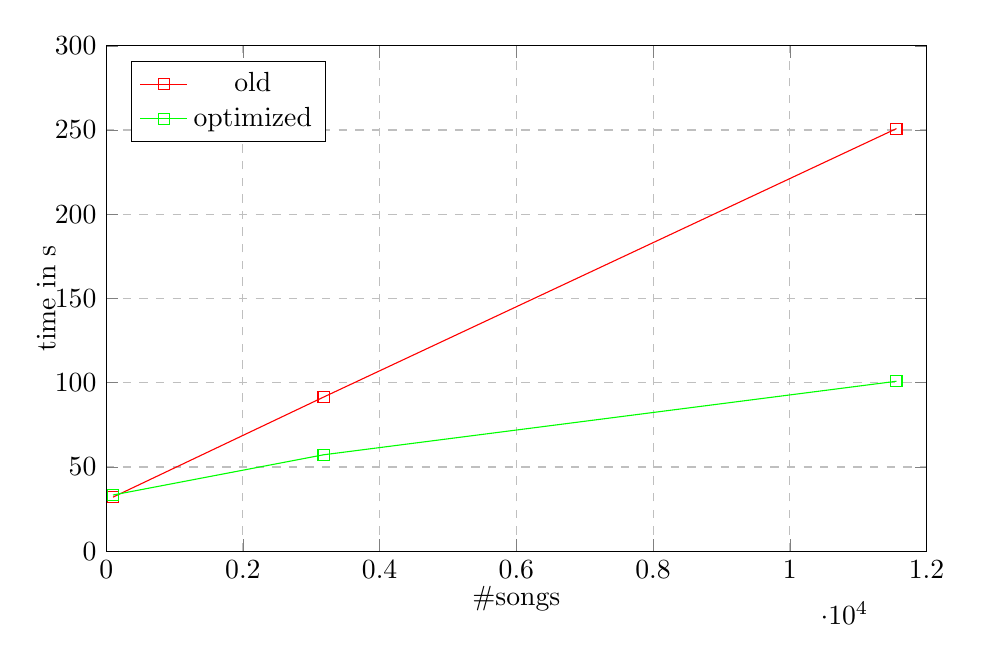
\begin{tikzpicture}
	\centering
	\begin{axis}[
	    %title={Performance of various toolkits},
		x label style={at={(axis description cs:0.5,-0.05)},anchor=north},
		y label style={at={(axis description cs:-0.05,.5)},rotate=0,anchor=south},
	    xlabel={\#songs},
	    ylabel={time in s},
	    xmin=0, xmax=12000,
	    ymin=0, ymax=300,
	    legend pos=north west,
	    ymajorgrids=true,
	    grid style=dashed,
	    height=8cm,
	    width=12cm,
	    grid=major,
	]
	%\addplot[color=red,mark=square,]
		%coordinates {(100,51.736)(3180,129.940)(11560,182.035)};
		%\addlegendentry{RDD cluster}
	%\addplot[color=blue,mark=square,]
	    %coordinates {(100,30.770)(3180,465.445)(11560,698.657)};
	    %\addlegendentry{RDD SN}
	\addplot[color=red,mark=square,]
	    coordinates {(100,32.087)(3180,91.477)(11560,250.854)};
	    \addlegendentry{old} 
	\addplot[color=green,mark=square,]
	    coordinates { (100,33.351)(3180,57.230)(11560,100.884)};
	    \addlegendentry{optimized}
	%\addplot[color=purple, mark=square,]
	    %coordinates {(100,13.874)(3180,34.232)(11560,78.566)};
	    %\addlegendentry{DataFrames unique SN}	    
	\end{axis}
	\end{tikzpicture}
	\caption{Performance single node(MFCC Euc, Notes, RP)}
	\label{perfspark1}
\end{figure}
\FloatBarrier

Why? Scaling of distances between 0 to 1 interval to combine different distances\\

\subsubsection{Combining different measurements}

weighted arithmetic mean of different distance measurements - there should be some kind of scaling \cite[pp. 543ff]{musicdata}\\

\begin{equation} \label{eq:distance}
dist = \frac{\sum_{m = 0}^{M - 1}{w_m \cdot d_m}}{\sum_{m = 0}^{M - 1}{w_m}}
\end{equation}

statistic prescaling to have mean = 0.5 and variance 0.5?\\


\subsection{performance}\label{sparkperf}

\subsubsection{Cluster configuration and data file size}

Memory intense - had to alter spark-defaults.conf\\

\begin{pythonCode}[frame=single,label={lst:clust},caption={cluster setup},captionpos=b]
confCluster = SparkConf().setAppName("MusicSimilarity Cluster")
confCluster.set("spark.driver.memory", "64g")
confCluster.set("spark.executor.memory", "64g")
confCluster.set("spark.driver.memoryOverhead", "32g")
confCluster.set("spark.executor.memoryOverhead", "32g")
confCluster.set("spark.yarn.executor.memoryOverhead", "4096")
confCluster.set("spark.driver.cores", "32")
confCluster.set("spark.executor.cores", "32")
confCluster.set("spark.dynamicAllocation.enabled", "True")
confCluster.set("spark.dynamicAllocation.minExecutors", "16")
confCluster.set("spark.dynamicAllocation.maxExecutors", "32")
confCluster.set("yarn.nodemanager.vmem-check-enabled", "false")
repartition_count = 32
\end{pythonCode}

\noindent FMA Many Small Files (40000 small files, 102000 songs)\\
MFCC + NOTES + RP:      {'TOTAL DF': 30517, 'TOTAL RDD': 211591, 'TOTAL MERGED': 39336}\\
JS + CHROMA + RP:       {'TOTAL DF': 32439, 'TOTAL RDD': 130989, 'TOTAL MERGED': 41490}\\                               
FMA ONE large file / feat (8 larger files, 102000 songs)\\
MFCC + NOTES + RP:      {'TOTAL DF': 33677, 'TOTAL RDD': 21933, 'TOTAL MERGED': 31963}\\
JS + CHROMA + RP:       {'TOTAL DF': 41477, 'TOTAL RDD': 35856, 'TOTAL MERGED': 51286}    
                                    

\subsubsection{Differences between the feature types}

Performance of similarity comparison with respect to lazy evaluation\\ 
Pre-merged with cached DataFrame containing all features - without loading data and without scaling.
Single DF = data loading + scaling 

\begin{figure}[htbp]
	\centering
	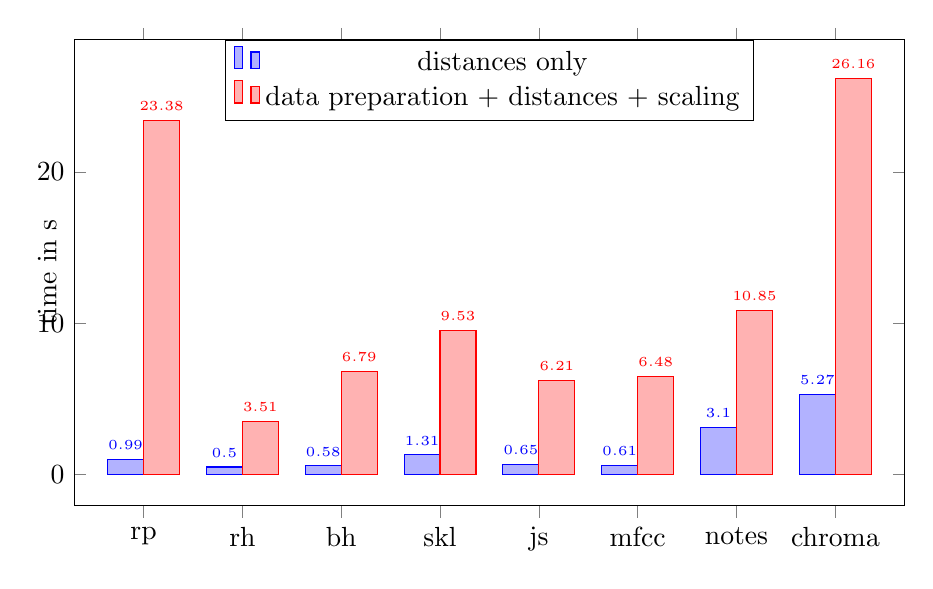
\begin{tikzpicture}
		\begin{axis}[
		    width=\textwidth,height=75mm,% <- added
		    x tick label style={/pgf/number format/1000 sep=0.05},
      		xticklabels={ , ,rp, rh, bh, skl, js, mfcc, notes, chroma}, 
		    ylabel=time in s,
  			y label style={at={(-0.01,0.5)}},
		    %enlargelimits=0.05,% <- commented, default is .1
		    legend style={
		      at={(0.5,1)},
		      anchor=north,% <- changed
		      %legend columns=-1% <- commented
		    },
		    nodes near coords,
		    every node near coord/.append style={font=\tiny},
		    %nodes near coords align={vertical},% <- commented, default
		    ybar=0pt,%<- changed
		    bar width=13pt% <- added
		  ]
		  \addplot
		    coordinates {(1,0.987) (2,0.504) (3,0.575) (4,1.306) (5,0.653) (6,0.613) (7,3.100) (8,5.273)};
		  \addplot
		    coordinates {(1,23.378) (2,3.506) (3,6.792) (4,9.527) (5,6.206) (6,6.475) (7,10.846) (8,26.160)};
		  \legend{distances only, data preparation + distances + scaling}
		\end{axis}
	\end{tikzpicture}
	\caption{Performance on different feature types}
	\label{features}
\end{figure}
\FloatBarrier

\subsubsection{Performance Comparison of RDD vs DataFrames vs single DataFrame}

Performance of optimized algorithms on the ARA-cluster\\
Merged DF = \\
DF = \\
RDD = \\
\ \\
\FloatBarrier
\begin{figure}[htbp]
	\centering
	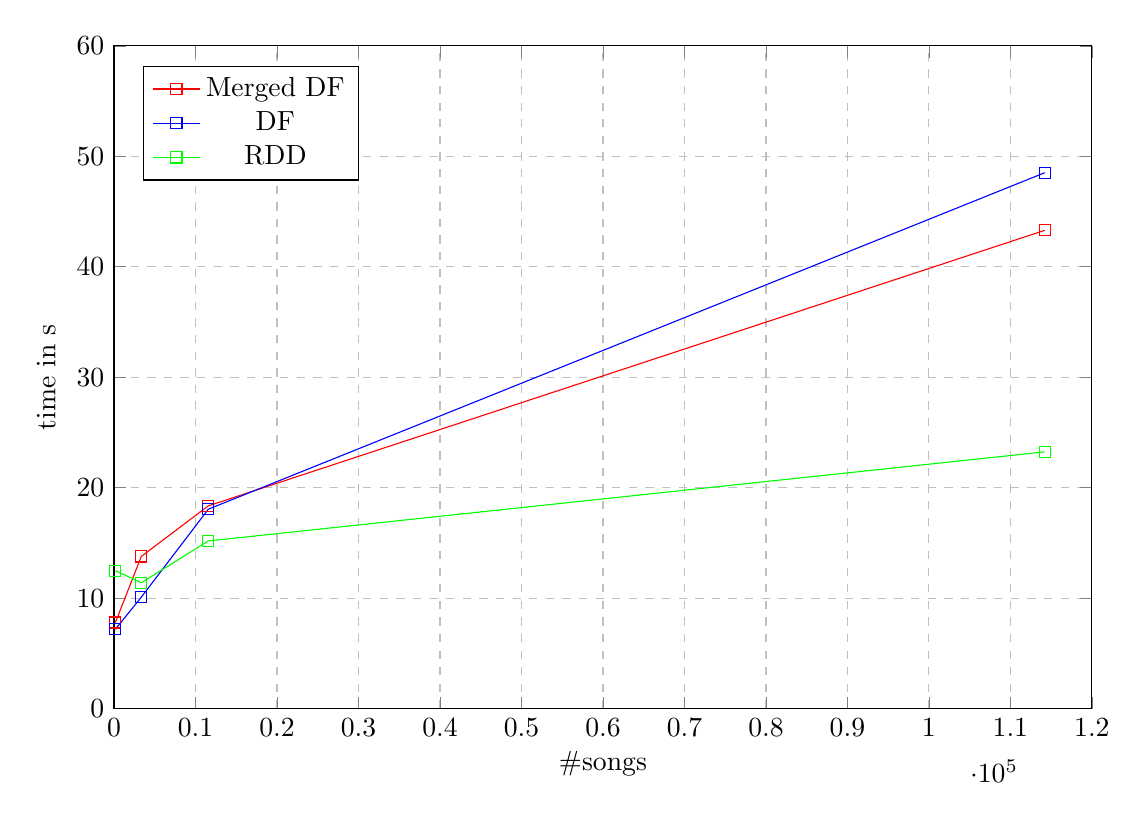
\begin{tikzpicture}
	\centering
	\begin{axis}[
	    %title={Performance of various toolkits},
		x label style={at={(axis description cs:0.5,-0.05)},anchor=north},
		y label style={at={(axis description cs:-0.05,.5)},rotate=0,anchor=south},
	    xlabel={\#songs},
	    ylabel={time in s},
	    xmin=0, xmax=120000,
	    ymin=0, ymax=60,
	    %xtick={0,1000,2000,3000,4000,5000,6000,7000,8000,9000,10000,100000,120000},
	    %ytick={0,100,200,300,400,500,600,700,800,900,1000},
	    legend pos=north west,
	    ymajorgrids=true,
	    grid style=dashed,
	    height=10cm,
	    width=14cm,
	    grid=major,
	]
	\addplot[color=red,mark=square,]
		coordinates {(164,7.800)(3344,13.778)(11564,18.356)(114210,43.296)};
		\addlegendentry{Merged DF}		
	\addplot[color=blue,mark=square,]
		coordinates {(164,7.189)(3344,10.090)(11564,18.052)(114210,48.512)};
		\addlegendentry{DF}	
	\addplot[color=green, mark=square,]
	    coordinates {(164,12.490)(3344,11.396)(11564,15.180)(114210,23.245)};
	    \addlegendentry{RDD}	  
	\end{axis}
	\end{tikzpicture}
	\caption{Performance ARA, full workload, (MFCC + Notes + RP)}
	\label{perfspark2}
\end{figure}
\FloatBarrier

\FloatBarrier
\begin{figure}[htbp]
	\centering
	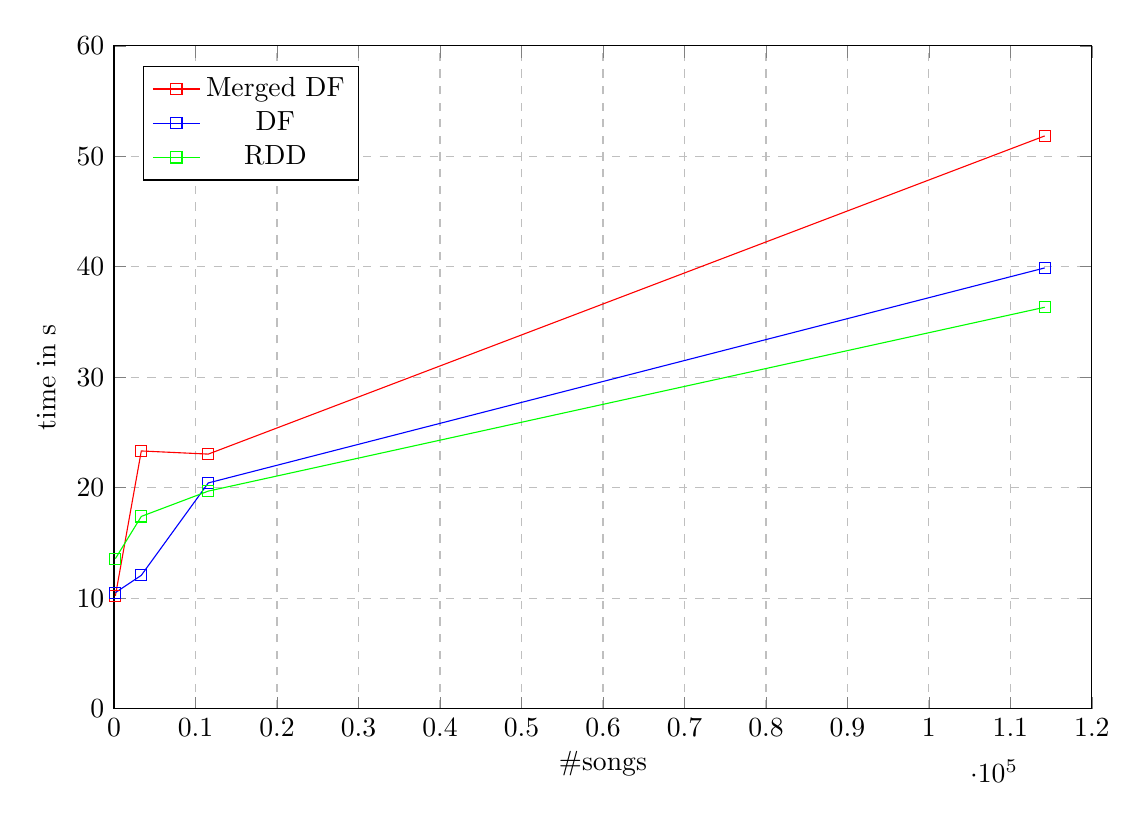
\begin{tikzpicture}
	\centering
	\begin{axis}[
	    %title={Performance of various toolkits},
		x label style={at={(axis description cs:0.5,-0.05)},anchor=north},
		y label style={at={(axis description cs:-0.05,.5)},rotate=0,anchor=south},
	    xlabel={\#songs},
	    ylabel={time in s},
	    xmin=0, xmax=120000,
	    ymin=0, ymax=60,
	    %xtick={0,1000,2000,3000,4000,5000,6000,7000,8000,9000,10000,100000,120000},
	    %ytick={0,100,200,300,400,500,600,700,800,900,1000},
	    legend pos=north west,
	    ymajorgrids=true,
	    grid style=dashed,
	    height=10cm,
	    width=14cm,
	    grid=major,
	]
	\addplot[color=red, mark=square,]
		coordinates {(164,10.208)(3344,23.327)(11564,23.042)(114210,51.842)};
		\addlegendentry{Merged DF}	
	\addplot[color=blue,mark=square,]
		coordinates {(164,10.506)(3344,12.069)(11564,20.432)(114210,39.894)};
		\addlegendentry{DF}
   	\addplot[color=green,mark=square,]
		coordinates {(164,13.580)(3344,17.401)(11564,19.692)(114210,36.334)};
		\addlegendentry{RDD}		
	\end{axis}
	\end{tikzpicture}
	\caption{Performance ARA, full workload, (JS + Chroma + RP)}
	\label{perfspark3}
\end{figure}
\FloatBarrier
    
\FloatBarrier
\begin{figure}[htbp]
   	\centering
   	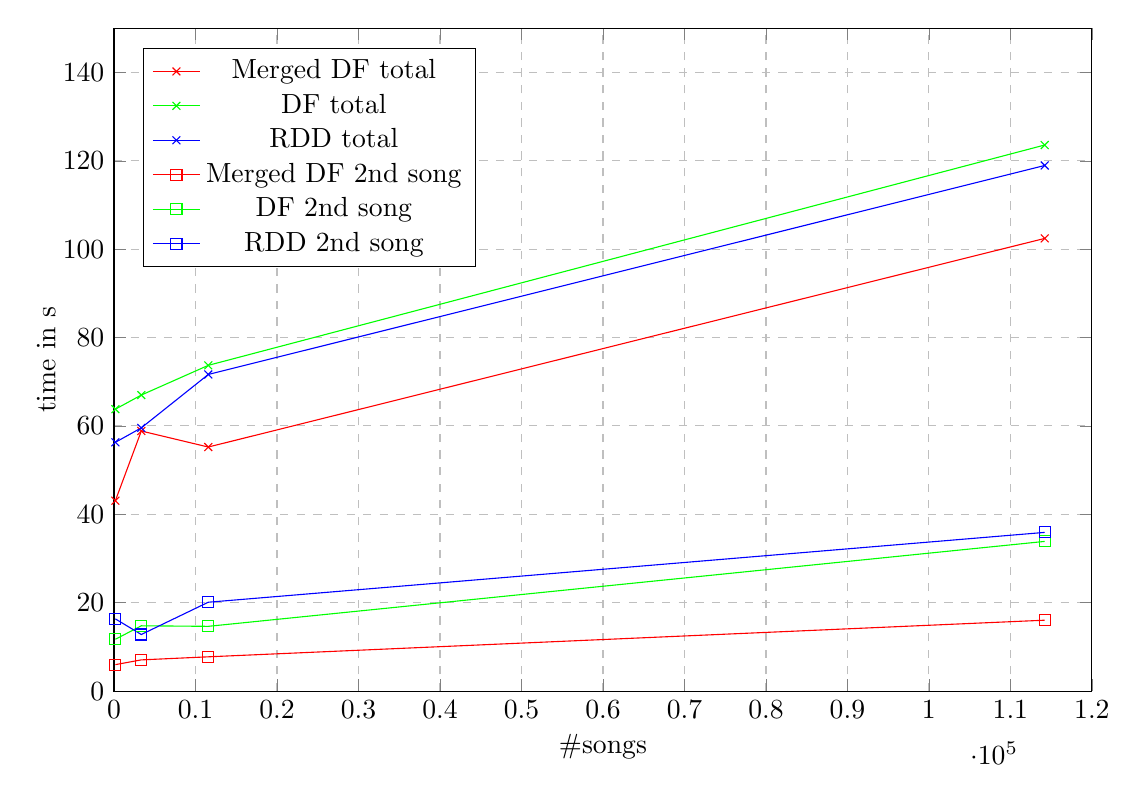
\begin{tikzpicture}
   	\centering
   	\begin{axis}[
	    %title={Performance of various toolkits},
   		x label style={at={(axis description cs:0.5,-0.05)},anchor=north},
   		y label style={at={(axis description cs:-0.05,.5)},rotate=0,anchor=south},
	    xlabel={\#songs},
	    ylabel={time in s},
	    xmin=0, xmax=120000,
	    ymin=0, ymax=150,
	    %xtick={0,1000,2000,3000,4000,5000,6000,7000,8000,9000,10000,100000,120000},
	    %ytick={0,100,200,300,400,500,600,700,800,900,1000},
	    legend pos=north west,
	    ymajorgrids=true,
	    grid style=dashed,
	    height=10cm,
	    width=14cm,
	    grid=major,
   	]
   	\addplot[color=red, mark=x,]
   		coordinates {(164,43.090)(3344,58.852)(11564,55.227)(114210,102.438)};
   		\addlegendentry{Merged DF total}
   	\addplot[color=green, mark=x,]
   		coordinates {(164,63.796)(3344,66.986)(11564,73.711)(114210,123.573)};
   		\addlegendentry{DF total}   		
   	\addplot[color=blue, mark=x,]
   		coordinates {(164,56.294)(3344,59.564)(11564,71.648)(114210,118.939)};
   		\addlegendentry{RDD total}   
   				
   	%\addplot[color=red, mark=x, dashed, dotted,]
   		%coordinates {(164,9.043)(3344,14.486)(11564,12.082)(114210,34.781)};
   		%\addlegendentry{Merged DF 1st song}   		
   	%\addplot[color=green, mark=x, dashed,]
   		%coordinates {(164,35.134)(3344,36.699)(11564,42.577)(114210,72.612)};
   		%\addlegendentry{DF 1st song}   		
   	%\addplot[color=blue, mark=x, dashed,]
   		%coordinates {(164,27.233)(3344,34.607)(11564,39.238)(114210,70.488)};
   		%\addlegendentry{RDD 1st song} 
 
   	\addplot[color=red, mark=square, ]
   		coordinates {(164,5.987)(3344,7.063)(11564,7.756)(114210,16.043)};
   		\addlegendentry{Merged DF 2nd song}   		
   	\addplot[color=green, mark=square,]
   		coordinates {(164,11.726)(3344,14.776)(11564,14.655)(114210,33.872)};
   		\addlegendentry{DF 2nd song}   		
   	\addplot[color=blue, mark=square,]
   		coordinates {(164,16.337)(3344,12.809)(11564,20.108)(114210,35.911)};
   		\addlegendentry{RDD 2nd song}   			
   	\end{axis}
   	\end{tikzpicture}
   	\caption{two subsequent songs, all features}
   	\label{perfspark4}
\end{figure}
\FloatBarrier

\subsection{possible performance improvements}

Pre- merge feature sets, broadcast comparator, descending importance pre-filtering\\
statistic normalization of similarities\\
Filter and refine after statistic normalization, drop all below mean\\
Is there a better way to cross-correlate???\\

\subsubsection{Descending Importance Filter and Refine}

Make use of caching from spark!\\
order of operations is important -> für elise chroma first actually better in cover song recognition\\

\FloatBarrier
\begin{figure}[htbp]
   	\centering
   	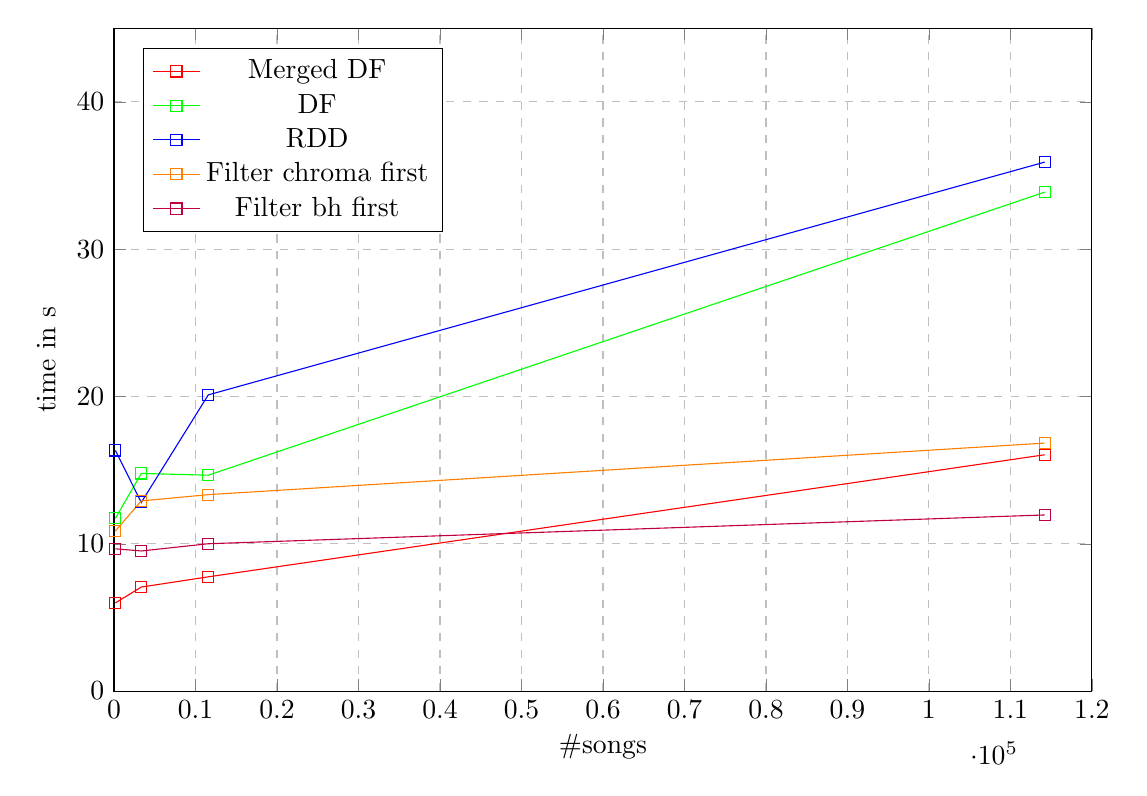
\begin{tikzpicture}
   	\centering
   	\begin{axis}[
	    x label style={at={(axis description cs:0.5,-0.05)},anchor=north},
   		y label style={at={(axis description cs:-0.05,.5)},rotate=0,anchor=south},
	    xlabel={\#songs},
	    ylabel={time in s},
	    xmin=0, xmax=120000,
	    ymin=0, ymax=45,
	    legend pos=north west,
	    ymajorgrids=true,
	    grid style=dashed,
	    height=10cm,
	    width=14cm,
	    grid=major,
   	]
   	%\addplot[color=red, mark=x,]
   	%	coordinates {(164,43.090)(3344,58.852)(11564,55.227)(114210,102.438)};
   	%	\addlegendentry{Merged DF total}
   	%\addplot[color=green, mark=x,]
   	%	coordinates {(164,49.274)(3344,59.691)(11564,65.949)(114210,94.464)};
   	%	\addlegendentry{Filter total}   		
   	\addplot[color=red, mark=square, ]
   		coordinates {(164,5.987)(3344,7.063)(11564,7.756)(114210,16.043)};
   		\addlegendentry{Merged DF}
  	\addplot[color=green, mark=square,]
  		coordinates {(164,11.726)(3344,14.776)(11564,14.655)(114210,33.872)};
  	   	\addlegendentry{DF}   		
  	\addplot[color=blue, mark=square,]
  		coordinates {(164,16.337)(3344,12.809)(11564,20.108)(114210,35.911)};
  		\addlegendentry{RDD}      		
   	\addplot[color=orange, mark=square,]
   		coordinates {(164,10.870)(3344,12.910)(11564,13.335)(114210,16.836)};
   		\addlegendentry{Filter chroma first}   
   	\addplot[color=purple, mark=square,]
   		coordinates {(164,9.658)(3344,9.512)(11564,10.002)(114210,11.957)};
   		\addlegendentry{Filter bh first}   					
   	\end{axis}
   	\end{tikzpicture}
   	\caption{Descending importance filter and refine, all features}
   	\label{perfspark5}
\end{figure}
\FloatBarrier

Merge total: 102.438\\
Filter total: 94.464\\

\subsubsection{Other alternatives}

Alternating Least Squares\\
TF-IDF weights\\
DIMSUM all-pairs similarity\\